\documentclass[master=ewit,english]{kulemt}
\setup{title={Building an end-to-end speech recognizer},
  author={Moritz Wolter},
  promotor={Prof.\,dr.\,ir.\ Johan Suykens \and Prof.\,dr.\,ir.\ Hugo Van hamme},
  assessor={Prof.\,dr.\,ir. Raf Vandenbrid \and Prof.\,dr.\,ir. Patrik Wambacq},
  assistant={Ir. Vincent Renkens}}
% The following \setup may be removed entirely if no filing card is wanted
\setup{filingcard,
  translatedtitle=,
  udc=621.3,
  shortabstract={
  	In the past machine learning relied heavily on algorithms designed by experts to solve a specific task. Which lead to highly sophisticated algorithms, which could be grasped only by small groups of people. The human brain however does not work this way, although specialized areas exist, these areas consist of similar
  	building blocks. Artificial neural networks attempt to mimic this layout. Similar algorithmic structures are used for a wide variety of tasks. This thesis deals with\ the application of neural networks in speech recognition. Replacing the various	subsystems by one integrated network based approach.
    \endgraf}}
% Uncomment the next line for generating the cover page
%\setup{coverpageonly}
% Uncomment the next \setup to generate only the first pages (e.g., if you
% are a Word user.
%\setup{frontpagesonly}

% Choose the main text font (e.g., Latin Modern)
\setup{font=lm}

% If you want to include other LaTeX packages, do it here.
% ---------- Titelblad Masterproef Faculteit Wetenschappen -----------
% Dit document is opgesteld voor compilatie met pdflatex.  Indien je
% wilt compileren met latex naar dvi/ps, dien je de figuren naar
% (e)ps-formaat om te zetten.
%                           -- december 2012
% -------------------------------------------------------------------
\RequirePackage{fix-cm}

% --------------------- In te laden pakketten -----------------------
% Deze kan je eventueel toevoegen aan de pakketten die je al inlaadt
% als je dit titelblad integreert met de rest van thesis.
% -------------------------------------------------------------------
\usepackage{graphicx,xcolor,textpos}

%----------------------- Custom stuff -------------------------------

\graphicspath{./}
\usepackage{makeidx}
\usepackage{amsmath}
\usepackage{amssymb}
\usepackage[english]{babel}
\usepackage{listings}
\usepackage{eurosym}
\usepackage{import}
\usepackage{multirow}
\usepackage{tabularx}


%------------------------ Plot packages ----------------------------
\usepackage{tikz}
\usetikzlibrary{positioning,arrows,calc}
\usepackage{pgfplots}
\usepackage{pgf}
\usepackage{units}
\usepackage{metalogo}
\usepackage{graphicx}
\usepackage{caption}
\usepackage{subcaption}
\usepackage[mode=buildnew]{standalone}% requires -shell-escape

% Finally the hyperref package is used for pdf files.
% This can be commented out for printed versions.
\usepackage[pdfusetitle,colorlinks,plainpages=false,hidelinks]{hyperref}


\begin{document}


\begin{preface}
	This thesis is about attention mechanisms in speech recognition. Attention allows artificial neural nets to focus on audio, video or text data. The concept is therefore not only important in speech processing. It also appears in amazing feats of engineering such a neural Turing machines \cite{Graves2014}, automatic translators \cite{Bahdanau2015} or self programming computers \cite{Neelakantan2016}. I hope you will enjoy reading about this exciting topic.
	
	I would like to thank my supervisor Vincent Renkens, for introducing me to the subject and the constant stream of good ideas and code he contributed to this project. I would like to extend my gratitude to my supervisor Prof. Van hamme for his feedback, debugging ideas, and for believing into this project even when nothing was working. Furthermore would like to thank everyone at the speech group in Leuven for their feedback during numerous lunch meetings and for granting me access to the group's computing power, without which this project would have been impossible.
	
	My sincere gratitude also goes to my parents for supporting me all the way trough my studies. 
	  
\end{preface}

\tableofcontents*

\begin{abstract}
  Speech recognition is concerned with transcribing what is said in a
  recoding of spoken language. In machine learning terms this process is
  called sequence labeling. A recoding consists of a chain of frames,
  this chain can be split up into several sequences, these make
  up words or phonemes, which must be labeled. The sequence of labels forms
  the transcription. \\
  The meaning of speech depends on context, therefore a good system needs to
  take it into account. Classical feed-forward networks fail to do that, which
  is why systems in this thesis will mainly consist of recurrently connected Long Short Term  Memory (LSTM) blocks. Inspired by the recurrent connections of neurons in the human brain, LSTM-RNNs have the ability to store information over long time periods. \\
  In order to train machine learning systems, speech and transcription text
  pairs are used. The text contains the exact information of what is said in
  the recording, but where in the recoding which word or sound is said is unknown.
  In other words text to speech alignment is missing. They key problem in this thesis is data alignment. Potential solutions such as connectionist temporal classification as well as attention based transducers will be discussed, with a focus on the latter.

\end{abstract}

% A list of figures and tables is optional
%\listoffigures
%\listoftables
% If you only have a few figures and tables you can use the following instead
\listoffiguresandtables
% The list of symbols is also optional.
% This list must be created manually, e.g., as follows:
\chapter{List of Abbreviations and Symbols}
\section*{Abbreviations}
\begin{flushleft}
  \renewcommand{\arraystretch}{1.1}
  \begin{tabularx}{\textwidth}{@{}p{12mm}X@{}}
    ASR   & Automatic speech recognition \\
    MLP	  & Multilayer perceptron \\
    CNN   & Convolutional neural network \\
    RNN   & Recurrent neural network \\
    LSTM  & Long short term memory \\
    BLSTM & Bidirectional long short term memory \\
    PLSTM & Pyramidal long short term memory \\
    LAS	  & Listen attend and spell
  \end{tabularx}
\end{flushleft}
\section*{Symbols}
\begin{flushleft}
  \renewcommand{\arraystretch}{1.1}
  \begin{tabularx}{\textwidth}{@{}p{12mm}X@{}}
	$\mathbf{f}$ & Mel feature vector \\
	$\mathbf{m}$ & Mean vector \\
	$\sigma$	 & Standard deviation vector \\
	$\mathbf{x}$ & System input vector \\
	$\hat{\mathbf{x}}$ & Standardized input vector \\
	$\hat{\mathbf{y}}$ & Label probability distribution vector \\
	$\mathbf{y}$ & Label output vector \\
	$E$			 & Cost function \\
	$\mathbf{w}$ & Model weight vector \\
	$\triangle$	 & Gradient \\
	$\mathbf{c}$  & LAS context vector \\
	$\mathbf{s}$  & Recurrent cell state \\
	$\mathbf{h}$  & Hidden value vector \\
	$\alpha$	 & Attention vector \\
	
  \end{tabularx}
\end{flushleft}

% Now comes the main text
\mainmatter

\import{chapters/}{problemStatement}
\import{chapters/}{literature}
\import{chapters/}{methodology}
\import{chapters/}{implementation}
\import{chapters/}{ctcExperiments}
\import{chapters/}{lasExperiments}
\import{chapters/}{conclusion}
% ... and so on until
%\import{../chapters/}{conclusion}


\backmatter
% The bibliography comes after the appendices.
% You can replace the standard "abbrv" bibliography style by another one.
\bibliographystyle{abbrv}
\bibliography{chapters/references}

% If you have appendices:
\appendixpage*          % if wanted
\appendix
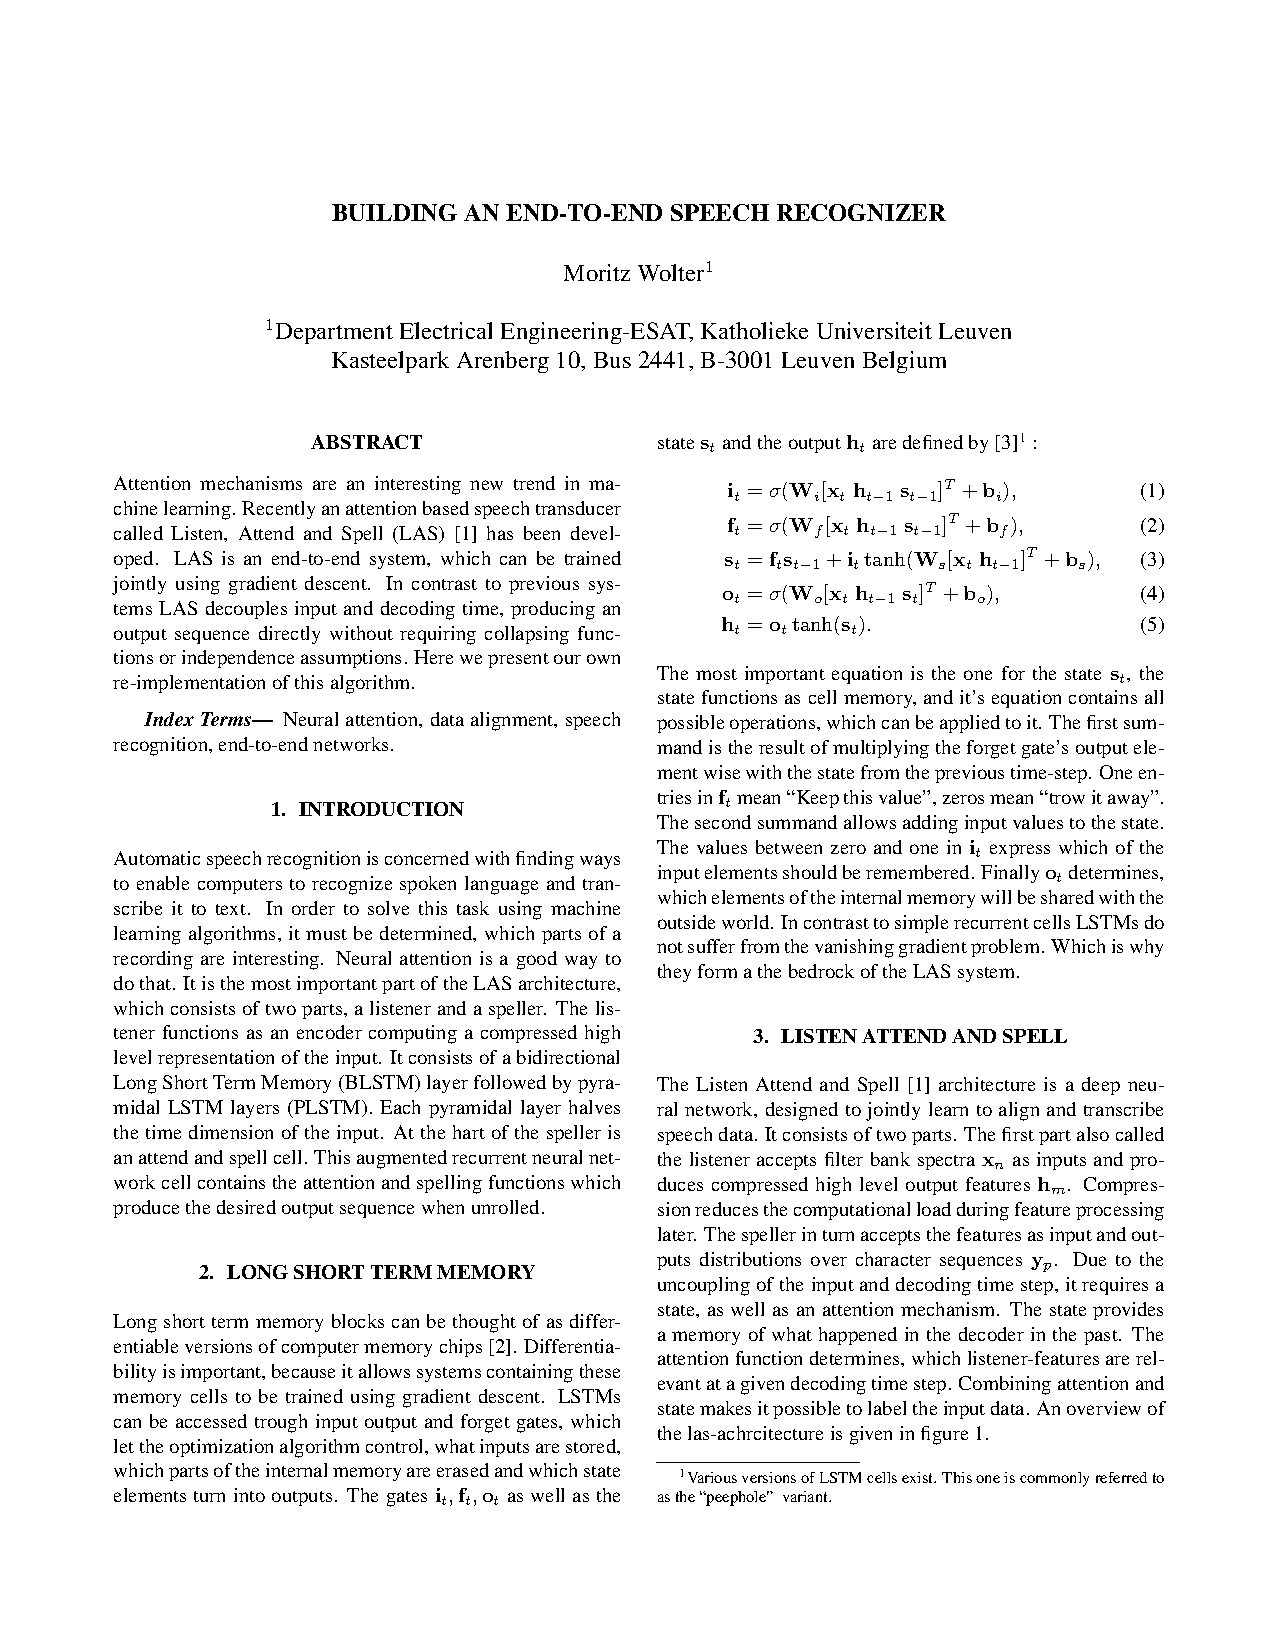
\includepdf[pages={1,2,3,4}]{paper/paperWolter.pdf}

\end{document}

%%% Local Variables:
%%% mode: latex
%%% TeX-master: t
%%% End:
